\sectionquestion{Decision Trees}

\begin{parts}

    \part The below $3\times 3$ tic-tac-toe board is actually a binary classification problem! Figure \ref{fig:tictactoe} shows a dataset containing 9 points: 5 labeled O and 4 labeled X. Suppose you want to build a decision tree, where each node splits based on one of these four lines: that is, one branch accepts points on one side of the line and one branch accepts points on the other side of that line.  (For full credit below, you must report the \emph{error rate}, not the number of errors.)

    \begin{figure}[H]
        \centering
        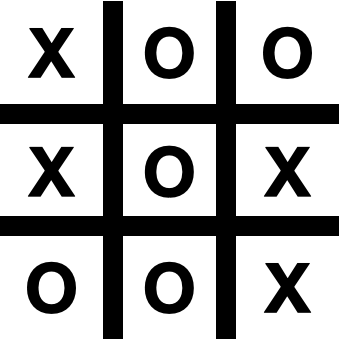
\includegraphics[width = 0.2\textwidth]{figures/tictactoe.png}
        \caption{"Tic-Tac-Toe" Dataset}
        \label{fig:tictactoe}
    \end{figure}

    \begin{subparts}
    \subpart[2] What is the minimum error rate we can achieve with a depth 1 decision tree on the above dataset (i.e. split on 1 line)? 
        \begin{tcolorbox}[fit,height=1cm, width=2cm, blank, borderline={1pt}{-2pt}]
        %solution
        \end{tcolorbox}
        \begin{soln}
        $\frac{3}{9}=\frac{1}{3}$
        \end{soln}

    \subpart[2] What is the minimum error rate we can achieve with a depth 2 decision tree? 
        \begin{tcolorbox}[fit,height=1cm, width=2cm, blank, borderline={1pt}{-2pt}]
        %solution
        \end{tcolorbox}
        \begin{soln}
        $\frac{1}{9}$
        \end{soln}

    \subpart[2] What is the minimum error rate we can achieve with a depth 3 decision tree?
        \begin{tcolorbox}[fit,height=1cm, width=2cm, blank, borderline={1pt}{-2pt}]
        %solution
        \end{tcolorbox}
        \begin{soln}
        $\frac{0}{9}$
        \end{soln}

    \begin{comment}
    \subpart[1] Let's generalize our results to any $N\times N$ tic-tac-toe dataset where each of the $N^2$ cells contains either 1 O or 1 X. The total count of each label does not matter. There is a linear decision boundary between every row and between every column. How deep must the decision tree be to guarantee 0 error rate?
        \begin{tcolorbox}[fit,height=1cm, width=2cm, blank, borderline={1pt}{-2pt}]
        %solution
        \end{tcolorbox}
        \begin{soln}
        $2(N-1)$. Consider a checkerboard pattern such as [O X O; X O X; O X O]. All decision boundaries are required to perfectly split the data. There are $N-1$ vertical decision boundaries and $N-1$ horizontal decision boundaries.
        \end{soln}

    \subpart[2] \textbf{Select one:} Which expression is equal to the entropy of the dataset in Figure 1?
        \begin{checkboxes}
            \choice $ -\frac{1}{9}\log_2{[\frac{5^5 4^4}{9}]} $
            \choice $ -\frac{1}{9^9}\log_2{[5^5 4^4]} $
            \choice $ -\log_2{[(\frac{5}{9})^5 (\frac{4}{9})^4]} $
            \choice $ -\frac{1}{9}\log_2{[(\frac{5}{9})^5 (\frac{4}{9})^4]} $
        \end{checkboxes}
        \begin{soln}
        D;
        $ H(Y) = -[\frac{5}{9}\log_2{\frac{5}{9}}
                + \frac{4}{9}\log_2{\frac{4}{9}}] 
                = -\frac{1}{9}[5\log_2{\frac{5}{9}}
                + 4\log_2{\frac{4}{9}}] 
                = -\frac{1}{9}log_2{
                [(\frac{5}{9})^5 (\frac{4}{9})^4] } $
        \end{soln}
    \end{comment}
    
    \subpart[3] \textbf{Select all that apply:} Which of the following would increase the entropy of label distribution for the training dataset in Figure \ref{fig:tictactoe}?
        {
        \checkboxchar{$\Box$} \checkedchar{$\blacksquare$}
        \begin{checkboxes}
            \choice Remove the center O.
            \choice Replace the center O with X. 
            \choice Remove the points in the top row.
            \choice Remove the points in the left column.
            % \choice Double the dataset (e.g. any cell containing O now has 2 Os).
            \choice Swap the points in the left column with the points in the middle column.
            \choice None of the above.
        \end{checkboxes}
        }
        \begin{soln}
            a) True. The ratio of O to X is now 4:4 = 1:1, resulting in the max entropy possible.\\
            b) False. The entropy would remain the same.\\
            c) True. The ratio of O to X is now 3:3 = 1:1, resulting in the max entropy possible.\\
            d) False. The ratio of O to X changes from 5:4 to 4:2. This ratio is further away from 1:1, meaning entropy would decrease instead.\\
            % e) False. The ratio of O to X remains the same at 10:8 = 5:4.\\
            e) False. Reordering the data does not affect entropy.
        \end{soln}
    
    \begin{qauthor}
    Author: Brandon Wang
    Objective: Use effective splitting criteria for Decision Trees and be able to define entropy, conditional entropy, and mutual information / information gain.
    
    Edited by Henry: truly awesome question, some parts removed for time. (d) is a bit too tricky for an exam, (e) is not really testing fundamental course concepts.
    \end{qauthor}
    \end{subparts}
        
    \begin{comment}
        \subpart[1] \textbf{True or False:} The resulting tree after pruning is guaranteed to have a lower test error than the original tree.
        \begin{checkboxes}
            \choice True 
            \choice False
        \end{checkboxes}
        \begin{soln}
            False
        \end{soln}
    \end{comment}
    
    \begin{qauthor}
        Hayden Kim
        
        Implement a pruning or early stopping method to combat overfitting in Decision Tree Learning (there are a LOT of recursion questions in OHs)
    \end{qauthor}

    \begin{qtester}
    EA Feedback: We should specify how we want them to fix it. E.g. "Identify the bug and write a line of pseudocode that would fix this mistake" or "Identify the bug and either describe in words or with pseudocode how to fix this mistake"

    Nice question
    \end{qtester}


\clearpage

\part Consider the training dataset in Figure \ref{fig:neuraldtreedata} consisting of 10 data points, where each point is labeled as either a square $y = \blacksquare$ or a triangle $y = \blacktriangle$.

\begin{figure}[h]
\begin{center}
    \begin{tikzpicture}
    \begin{axis}[
        scale=0.9, width=12cm, height=8cm, mark options={scale=1.7},
        xmin=0, xmax=10, xtick={1,2,3,4,5,6,7,8,9},
        ymin=0, ymax=6, ytick={1,2,3,4,5},
        samples=50, xlabel=$x_1$, ylabel=$x_2$]]
        \addplot [
            scatter,
            only marks,
            point meta=explicit symbolic,
            scatter/classes={
                a={mark=triangle*,red},
                b={mark=square*,blue}
            },
            nodes near coords*={},
            visualization depends on={\thisrow{myvalue} \as \myvalue},
        ] table [meta=label] {
            x y label myvalue
            1 4 b 1
            1 5 b 1
            2 1 a 1
            4 2 a 1
            6 1 a 1
            7 4 a 1
            7 5 a 1
            7 1 b 1
            8 2 b 1
            9 1 b 1
        };
    \end{axis}
    \end{tikzpicture} 
\end{center}
    \caption{}
    \label{fig:neuraldtreedata}
\end{figure}

Given this training dataset, Neural the Narwhal decides to use the decision tree in Figure \ref{fig:neuraldtree}.

\begin{figure}[h!]
    \def\splitDist{4cm}
    \def\rootDist{2.5cm}
    \centering
    \begin{tikzpicture}[
            scale=0.8,
            node/.style = {draw, rectangle},
            oval/.style = {ellipse, draw, inner xsep=#1},
            > = stealth, % arrow head style
            shorten > = 0pt, % don't touch arrow head to node
            auto,
            thick % line style
        ]

        \node[node] (S1) {$x_1 < 3$};
        \path (S1) ++(-135:\splitDist) node [node] (S2) {$x_2 < 3$};
        \path (S1) ++(-45:\splitDist) node [node] (S3) {$x_1 < 5$};
        \path (S2) ++(-135:\rootDist) node [oval] (L1) {$\blacktriangle$};
        \path (S2) ++(-45:\rootDist) node [oval] (L2) {$\blacksquare$};
        \path (S3) ++(-135:\rootDist) node [oval] (L3) {$\blacktriangle$};
        \path (S3) ++(-45:\splitDist) node [node] (S4) {$x_2 < 3$};
        \path (S4) ++(-135:\rootDist) node [oval] (L4) {$\blacksquare$};
        \path (S4) ++(-45:\rootDist) node [oval] (L5) {$\blacktriangle$};
    
        \draw (S1) -- (S2) node [left,pos=0.25] {true};
        \draw (S1) -- (S3) node [right,pos=0.25] {false};
        \draw (S2) -- (L1) node [left,pos=0.25] {true};
        \draw (S2) -- (L2) node [right,pos=0.25] {false};
        \draw (S3) -- (L3) node [left,pos=0.25] {true};
        \draw (S3) -- (S4) node [right,pos=0.25] {false};
        \draw (S4) -- (L4) node [left,pos=0.25] {true};
        \draw (S4) -- (L5) node [right,pos=0.25] {false};
    \end{tikzpicture}
    \caption{Neural's decision tree}
    \label{fig:neuraldtree}
\end{figure}

\begin{subparts}
\subpart[4] \textbf{Drawing:} On Figure \ref{fig:neuraldtreedata}, draw the decision boundary corresponding to Neural's decision tree. For full credit, you must shade in the region(s) labeled as $y=\blacksquare$.

\begin{soln}
\begin{center}
    \begin{tikzpicture}
    \begin{axis}[
        scale=1.2, width=12cm, height=8cm, mark options={scale=1.7},
        xmin=0, xmax=10, xtick={1,2,3,4,5,6,7,8,9},
        ymin=0, ymax=6, ytick={1,2,3,4,5},
        samples=50, xlabel=$x_1$, ylabel=$x_2$]]
        \addplot[red, ultra thick, dotted] coordinates { (0,3) (3,3) };
        \addplot[red, ultra thick, dotted] coordinates { (3,3) (3,6) };
        \addplot[red, ultra thick, dotted] coordinates { (5,0) (5,3) };
        \addplot[red, ultra thick, dotted] coordinates { (5,3) (10,3) };
        \addplot [
            scatter,
            only marks,
            point meta=explicit symbolic,
            scatter/classes={
                a={mark=triangle*,red},
                b={mark=square*,blue}
            },
            nodes near coords*={},
            visualization depends on={\thisrow{myvalue} \as \myvalue},
        ] table [meta=label] {
            x y label myvalue
            1 4 b 1
            1 5 b 1
            2 1 a 1
            4 2 a 1
            6 1 a 1
            7 4 a 1
            7 5 a 1
            7 1 b 1
            8 2 b 1
            9 1 b 1
        };
    \end{axis}
    \end{tikzpicture} 
\end{center}
\end{soln}
\begin{qauthor}
    Henry
\end{qauthor}

\subpart[2] \textbf{Numerical answer:} What is the training error rate of Neural's decision tree?
\begin{tcolorbox}[fit,height=1cm, width=2cm, blank, borderline={1pt}{-2pt}]
%solution
\end{tcolorbox}
\begin{soln}
    1/10
\end{soln}
\begin{qauthor}
    Henry
\end{qauthor}

% REMOVED FOR TIME
% \subpart[2] \textbf{Drawing:} In the space provided below, draw a decision tree with a depth of 2 that uses only features of the form $x_i < c$ and has the same decision boundary as Neural's decision tree.
% \begin{tcolorbox}[fit,height=6cm, width=15cm, blank, borderline={1pt}{-2pt}]
%     %solution
% \end{tcolorbox}
% \begin{soln}
%     \begin{figure}[h!]
%         \def\splitDist{3.5cm}
%         \def\rootDist{2.5cm}
%         \centering
%         \begin{tikzpicture}[
%                 node/.style = {draw, rectangle},
%                 oval/.style = {ellipse, draw, inner xsep=#1},
%                 > = stealth, % arrow head style
%                 shorten > = 0pt, % don't touch arrow head to node
%                 auto,
%                 thick % line style
%             ]
    
%             \node[node] (S1) {$x_2 < 3$};
%             \path (S1) ++(-135:\splitDist) node [node] (S2) {$x_1 < 3$};
%             \path (S1) ++(-45:\splitDist) node [node] (S3) {$x_1 < 5$};
%             \path (S2) ++(-135:\rootDist) node [oval] (L1) {$-1$};
%             \path (S2) ++(-45:\rootDist) node [oval] (L2) {$+1$};
%             \path (S3) ++(-135:\rootDist) node [oval] (L3) {$-1$};
%             \path (S3) ++(-45:\rootDist) node [oval] (L4) {$+1$};
        
%             \draw (S1) -- (S2) node [left,pos=0.25] {true};
%             \draw (S1) -- (S3) node [right,pos=0.25] {false};
%             \draw (S2) -- (L1) node [left,pos=0.25] {true};
%             \draw (S2) -- (L2) node [right,pos=0.25] {false};
%             \draw (S3) -- (L3) node [left,pos=0.25] {true};
%             \draw (S3) -- (L4) node [right,pos=0.25] {false};
%         \end{tikzpicture}
%     \end{figure}
% \end{soln}
% \begin{qauthor}
%     Henry
% \end{qauthor}
\end{subparts}

\part Your friend Wally is trying to build a decision tree to predict whether or not an object is trash. He gathers the following dataset, consisting of three features: Color (Green, Brown or Clear), Sound (either Crinkly or None) and Weight (High, Medium or Low). 

\begin{center}
    \begin{tabular}{ccc | c}
		\hline
		Color & Sound & Weight & Trash? \\
	    \hline
		Clear & None & High & No \\
		Clear & None & Medium & Yes \\
		Green & None & Medium & No \\ 
		Brown & Crinkly & High & Yes \\
		Green & Crinkly & Low & Yes \\
		Brown & Crinkly & Low & No \\ 
		\hline
    \end{tabular}
\end{center}

\begin{subparts}
\subpart[2] \textbf{Select one:} Given this dataset, which feature would the ID3 algorithm split on first? \textbf{Hint:} you should be able to solve this problem without needing to take any logarithms. 
\begin{checkboxes}
    \choice Color 
    \choice Sound
    \choice Weight
    \choice tie between Color and Sound 
    \choice tie between Color and Weight
    \choice tie between Sound and Weight
\end{checkboxes}
\begin{soln}
    B, both of the other features have $0$ information gain. 
\end{soln}
\begin{qauthor}
    Henry
\end{qauthor}	

\subpart[1] \textbf{True or False:} \emph{On this trash identification dataset}, the ID3 algorithm will return the shortest possible decision tree that achieves zero training error rate, regardless of how ties are broken. %\textbf{Briefly justify your answer in 1-2 concise sentences.}
\begin{checkboxes}
    \choice True 
    \choice False
\end{checkboxes}
%\fillwithlines{6em}
\begin{soln}
    False, after splitting on Sound, there is no subsequent split that can perfectly classify the dataset. However, splitting on either Color or Weight first, you can perfectly classify the dataset by then splitting on the other. 
\end{soln}
\begin{qauthor}
    Henry 
\end{qauthor}		  
\end{subparts}

\begin{comment}	  
\part[2] \textbf{True or False:} Given a training dataset $\mathcal{D}$ of finite size with binary labels, there always exists a decision tree that can achieve zero training error on $\mathcal{D}$. \textbf{Briefly justify your answer in 1-2 concise sentences.}
\begin{checkboxes}
    \choice True 
    \choice False
\end{checkboxes}
\fillwithlines{6em}
\begin{soln}
    False. If there are two training examples that have the same feature values but different labels, then a decision tree can never get them both right. 
\end{soln}
\begin{qauthor}
    Henry
\end{qauthor}
\end{comment}

\part[3] \textbf{Short answer:} Suppose you are given a dataset $\mathcal{D}$. In 3-5 concise sentences, describe a procedure in which you (1) partition $\mathcal{D}$ into some number of disjoint subsets, (2) learn a decision tree using the ID3 algorithm, (3) determine whether you should or should not prune the learned decision tree, and (4) evaluate the resultant tree. In order to receive full credit, you must specify the number and name of the disjoint subsets you partition $\mathcal{D}$ into and follow proper experimental design principles. 
\fillwithlines{10em}
\begin{soln}
    One possible solution would be to split $\mathcal{D}$ into $\mathcal{D}_{\textrm{train}} \cup \mathcal{D}_{\textrm{val-1}} \cup \mathcal{D}_{\textrm{val-2}} \cup \mathcal{D}_{\textrm{test}}$
    Train a decision tree using the ID3 algorithm on $\mathcal{D}_{\textrm{train}}$. Then, duplicate this tree and prune one of the copies using $\mathcal{D}_{\textrm{val-1}}$. Compute the validation error of the pruned tree and the original tree on using $\mathcal{D}_{\textrm{val-2}}$. If the pruned tree achieves a lower validation error on $\mathcal{D}_{\textrm{val-2}}$, conclude that you should apply pruning in this setting. (OPTIONAL) Finally, estimate the true error of whichever tree did best on $\mathcal{D}_{\textrm{val-2}}$ using $\mathcal{D}_{\textrm{test}}$. 
    
    We should be open to other solutions e.g., ones that omit $\mathcal{D}_{\textrm{test}}$. 
\end{soln}
\begin{qauthor}
    Henry
\end{qauthor}

\begin{comment}
\part[3] \textbf{Short answer:} Suppose you are given a dataset that is partitioned into \emph{four} disjoint datasets, $\mathcal{D} = \mathcal{D}_{\textrm{train}} \cup \mathcal{D}_{\textrm{val-1}} \cup \mathcal{D}_{\textrm{val-2}} \cup \mathcal{D}_{\textrm{test}}$. In 3-5 concise sentences, describe a procedure using these four datasets that would allow you to determine whether or not you should prune a decision tree learned using the ID3 algorithm on this dataset. 
\fillwithlines{12em}
\begin{soln}
    First train a decision tree using the ID3 algorithm on $\mathcal{D}_{\textrm{train}}$. Then, duplicate this tree and prune one of the copies using $\mathcal{D}_{\textrm{val-1}}$. Compute the validation error of the pruned tree and the original tree on using $\mathcal{D}_{\textrm{val-2}}$. If the pruned tree achieves a lower validation error on $\mathcal{D}_{\textrm{val-2}}$, conclude that you should apply pruning in this setting. (OPTIONAL) Finally, estimate the true error of whichever tree did best on $\mathcal{D}_{\textrm{val-2}}$ using $\mathcal{D}_{\textrm{test}}$. 
\end{soln}
\begin{qauthor}
    Henry; AUTHOR'S NOTE: does providing the partitioning into four datasets make this question too easy?
\end{qauthor}
\end{comment}

\end{parts}
